% -*- TeX-master: "main" -*-

\section{Package syntax and semantics}
\label{syntax}

This section contains a definition of the syntax and semantics of the Required Element package for \sbmlthreecore.  

% --------------------------------------------------------------------------
\subsection{Namespace URI and other declarations necessary for using this package}
\label{xml-namespace}

Every SBML Level~3 package is identified uniquely by an XML namespace URI.  For an SBML document to be able to use a given Level~3 package, it must declare the use of that package by referencing its URI.  The following is the namespace URI for this version of the Required Elements package for \sbmlthreecore:
\begin{center}
\uri{http://www.sbml.org/sbml/level3/version1/groups/version1}
\end{center}

In addition, SBML documents using a given package must indicate whether understanding the package is required for complete mathematical interpretation of a model.  This is done using the attribute \token{required} on the \token{<sbml>} element in the SBML document.  For the Required Elements package, the value of this attribute must be \val{false}, because the use of the Required Elements package cannot change the mathematical meaning of a model.

The following fragment illustrates the beginning of a typical SBML model using \sbmlthreecore and this version of the Required Elements package:

\begin{example}
<?xml version="1.0" encoding="UTF-8"?>
<sbml xmlns="http://www.sbml.org/sbml/level3/version1/core" level="3" version="1"
      xmlns:req="http://www.sbml.org/sbml/level3/version1/groups/version1" req:required="false">
\end{example}


\subsection{Primitive data types}
\label{new-primitive-types}

The Required Elements package uses two of the primitive data types described in Section~3.1 of the \sbmlthreecore specification, specifically \primtype{string} and \primtype{boolean}.  The package does not define any new types.


\subsection{The extended \class{SBase} class}
\label{extended-sbase-class}

As mentioned above, this package's reason for being is to define two optional attributes on the SBML Level~3 \SBase class.  \fig{extended-sbase-uml} provides the definition of this extended \SBase class.  These attributes are added to \SBase instead of to those elements that have math in them (such as \Parameter, \Species, etc.) because this approach allows other SBML Level~3 packages to define new elements with mathematics which may, in turn be overridden by other packages.

\begin{figure}[bh]
  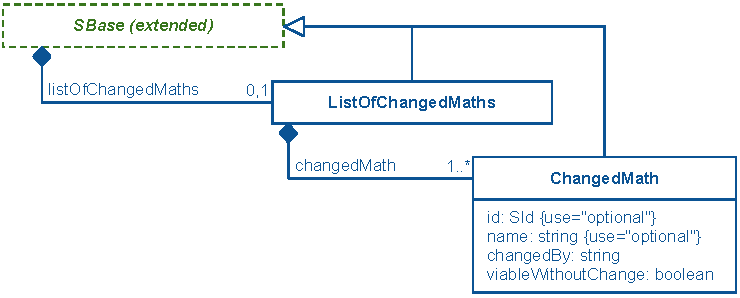
\includegraphics{figs/extended-sbase-req-uml}
  \vspace*{-3.5em}
  \caption{The definition of the extended \SBase class.}
  \label{extended-sbase-uml}
\end{figure}

\subsubsection{The \fixttspace\tokenNC{mathOverridden} attribute}
\label{attribute-mathoverridden}

The first attribute added to \SBase is \token{mathOverriden}.  Its value type is \token{string}.  When set, the attribute must be set to the namespace URI of the SBML Level~3 package that redefines the mathematical semantics of the object on which the attribute is set.  In other words, if the mathematical semantics of a given component \emph{C} in a model is changed by the use of a Level~3 package \emph{P}, then \emph{C} can be given the attribute \token{mathOverridden} and the value of that attribute should be \emph{P}'s namespace URI.  The examples below will make this more clear.

Note that the \token{mathOverridden} attribute should be placed on the model component that is directly affected, and not on a component that is indirectly affected by the changed mathematics.  For example, if a model contains a \FunctionDefinition object whose mathematics are extended by the SBML Level~3 package for Distributions, and in addition, elsewhere in the model there is an \InitialAssignment object that uses the function, the \token{mathOverridden} attribute must be added only on the \FunctionDefinition object and not the \InitialAssignment, because the latter is only indirectly affected.


\subsubsection{The \fixttspace\tokenNC{coreHasAlternativeMath} attribute}
\label{attribute-corehasalternativemath}

The second attribute added to \SBase is \token{coreHasAlternativeMath}.  Its value type is \token{boolean}.  The attribute should be set to \val{true} or \val{false} depending on whether an interpreter that \emph{only} understands \sbmlthreecore would have a workable and complete (if perhaps different) version of the mathematics for a given component in a model.  ``Complete understanding'' is an objective requirement for setting this attribute to \val{true}---the Level~3 Core parts of the component must not leave any of the mathematics undefined.  ``Workable'' requires a judgement call on the part of the modeler: if the modeler feels that the alternative version makes sense in an alternative context, they may set the attribute value to \val{true}; conversely, if they feel that the resulting model component makes no sense, even if technically ``complete'', then they should set the attribute value to \val{false}.


\subsection{Additional considerations}

The Required Elements package is not, itself, required (that is, models that use it must set \token{required}=\val{false} for its namespace when using it) because it, in and of itself, does not change any mathematical semantics.  However, it is intended to be used by other required packages, which may in turn make the use of one or both attributes from this package required in certain contexts defined in those package specifications. For example, the Spatial Processes package could require that modelers set the attribute \token{mathOverridden}=\val{distrib} for any reactions whose kinetic laws were redefined by that package. This would provide a clean way of ensuring that only one package overrode the math for any single SBML component: if two packages required the \token{mathOverridden} attribute to be set to their own namespace, it would be impossible to doubly-override a single element without failing to comply with at least one package specification.

It is possible that future versions of SBML Level~3 may incorporate the constructs of the Required Elements package directly into the Core specification itself, should this prove generally useful.
